\chapter{Dinámica de los sistemas de partículas}
\chaptermark{Dinámica sistemas partículas}

\begin{miparrafo}
Una partícula es una entidad física que posee masa pero carece de dimensiones geométricas.

Para un cuerpo real se nos presenta una dificultad. Cualquiera de las partículas que forman el cuerpo puede estar sometida a una fuerza exterior debido a la posición que ocupa en el universo y también sometido a una fuerza interior debida a las propias partículas que forman el cuerpo. (En $1 \text{mm}^3$ de líquido hay $\sim 10^{24}$ partículas, tendríamos una ingente cantidad de ecuaciones que plantear).

La aproximación de punto material es válida en los movimientos de traslación y en aquellos casos en los que la precisión en la localización del cuerpo es del orden de las dimensiones de éste. Por tanto, hay de proponer un nuevo modelo que permita estudiar los cuerpos, y su evolución temporal, en los casos en que la aproximación anterior no sea válida. Este modelo es el de \emph{sistemas de partículas:  un conjunto de partículas cuyas propiedades globales queremos estudiar}. 

Los sistemas de partículas se pueden clasificar en:
\begin{itemize}
	\item Sistema discreto, cuando el cuerpo se considera formado por un número finito de partículas. Dentro de este modelo podemos considerar:
		\begin{itemize}
		\item Sistemas indeformables, en los que la distancia relativa entre las partículas del sistema permanece inalterable en el tiempo.
		\item Sistemas deformables, en los que puede cambiar la distancia relativa entre las partículas.
		\end{itemize}
	\item Sistemas continuos, cuando un cuerpo puede considerarse formado por una distribución “continua” de materia (llenando todo el espacio que ocupa). Estos sistemas se dividen en deformables e indeformables (sólidos rígidos).
\end{itemize}
Vamos a estudiar si las magnitudes importantes para la física se conservan o no para el sistema de partículas.
\end{miparrafo}

\section[Teorema de conservación de la cantidad de movimiento. Sistema de referencia centro de masas y de laboratorio]{Teorema de conservación de la cantidad de movimiento. Sistema de referencia centro de masas y de laboratorio\sectionmark{Conservación cantidad de movimiento}}
\sectionmark{Conservación cantidad de movimiento}

Consideremos un sistema formado por $N$ partículas y sea $\vec F_i^{(e)}$ la fuerza externa que actúa sobre la partícula $i$. La fuerza que ejercen el resto de partículas, $N-1$, sobre la partícula $i$ es:

$\vec F_{i1}+\vec F_{2i}+ \cdots + \vec F_{(N-1)i}+\vec F_{(N+1)i}+ \cdots +\vec F_{Ni}$

Aplicando la segunda ley de Newton:

$\vec F_i^{(e)}\ + \ \vec F_{i1}+\vec F_{2i}+ \cdots + \vec F_{(N-1)i}+\vec F_{(N+1)i}+ \cdots +\vec F_{Ni}=\displaystyle \dv{\vec p_i}{t}$

Esquemáticamente: $\ \displaystyle \dv{\vec p_i}{t}= \sum_{\substack{j=1 \\ j\neq i}}^{N} \vec F_{ji} \ + \ \vec F_i^{(e)}$

Para las $N$ partículas habrá que resolver $N$ ecuaciones como esta. Sumándolas todas:$\quad \displaystyle \dv{t} \sum_{i=1}^N \vec p_i = \sum_i \sum_j \vec F_{ji}+\sum_i \vec F_i^{(e)}$

Suponiendo que se cumple la ley de acción-reacción, $\vec F_{ji}=-\vec F_{ij}$, por tanto, $\quad \displaystyle \sum_i \sum_j \vec F_{ji}=0$ y, finalmente:

\begin{equation}
\subrayado{\ \boxed{ \boldsymbol{ \dv{\vec P}{t}=\vec F^{(e)}}\ }\ } \qquad \text{ con } \vec F^{(e)}=\sum_i	\vec F_i^{(e)} \ \  \text{ y } \ \ \vec P=\sum_i \vec p_i
\end{equation}

Expresión que se conoce como \subrayado{\emph{``Teorema de la cantidad de movimiento''}} y viene a decir que:

\begin{miparrafodestacado}
	 \emph{`un sistema de partículas evoluciona de idéntica forma a lo que lo haría una partícula sobre la que actuase una fuerza externa'.}
\end{miparrafodestacado}


Cuando las coordenadas  que usamos son las del laboratorio se dice que estamos usando el \emph{sistema de referencia de laboratorio}.

Al igual a lo que pasaba para una partícula, para un sistema de partículas, si $ \subrayado{\vec F^{(e)}=\vec 0 \ \to \ \displaystyle \sum_i \vec p_i=\overrightarrow{cte}}$

Vamos a introducir un nuevo sistema de referencia, el \emph{\textbf{sistema de referencia centro de masas}}.

\begin{miparrafodestacado}
El centro de masas, $CM$, de un sistema de $N$ partículas es, por definición, aquel punto del espacio que tiene un vector de posición $\vec R$ que viene determinada por la siguiente expresión:	
\end{miparrafodestacado}

\begin{equation}
\subrayado{\boldsymbol{ \vec R=\dfrac 1 M \ \sum_{i=1}^{N} m_i \ \vec r_i}}
\end{equation}

siendo $\vec r_i$ el vector de posición de la partícula $i$ respecto del origen $\mathcal{O}$ que hayamos tomado.

Veamos como evoluciona el $CM$ respecto al tiempo:

\begin{equation}
\subrayado{\boldsymbol{\vec v_{CM}=\dv{\vec R}{t}}}= \dfrac 1 M \ \sum_{i=1}^N m_i\ \vec v_i=\frac 1 M \sum_{i=1}^N \vec p_i= \subrayado{ \boldsymbol{\dfrac {\vec P}{M}}}
\end{equation}

Aplicando el \emph{teorema de la cantidad de movimiento},

\begin{equation}
\subrayado{\ \boxed{\ \boldsymbol{M\ \dv{\vec v_{CM}}{t}}\ =\ \vec F^{(e)}  \ } \ }	
\end{equation}

\begin{miparrafodestacado}
\emph{El $CM$ de un sistema de partículas se comporta como si se tratase de una partícula de masa $M$ igual a la masa total del sistema y que se desplaza con la velocidad del centro de masas, $\vec v_{CM}$	}
\end{miparrafodestacado}

\emph{Un \textbf{sistema} $\boldsymbol{CM}$ es un sistema de referencia centrado en el $CM$}

Obviamente, si estamos en el $CM$, la velocidad respecto al centro de masas $\vec v_{CM}=0$
Si  $\vec v_{CM}=\frac {\vec P}{M}=0 \ to \ \vec P=\sum_i \vec p_i=0$,
lo que da una nueva definición al centro de masas: es aquel punto del espacio en que $\sum_i \vec p_i=0=\sum_i m_i\ \vec v_{i, \ CM}$.

\begin{figure}[H]
	\centering
	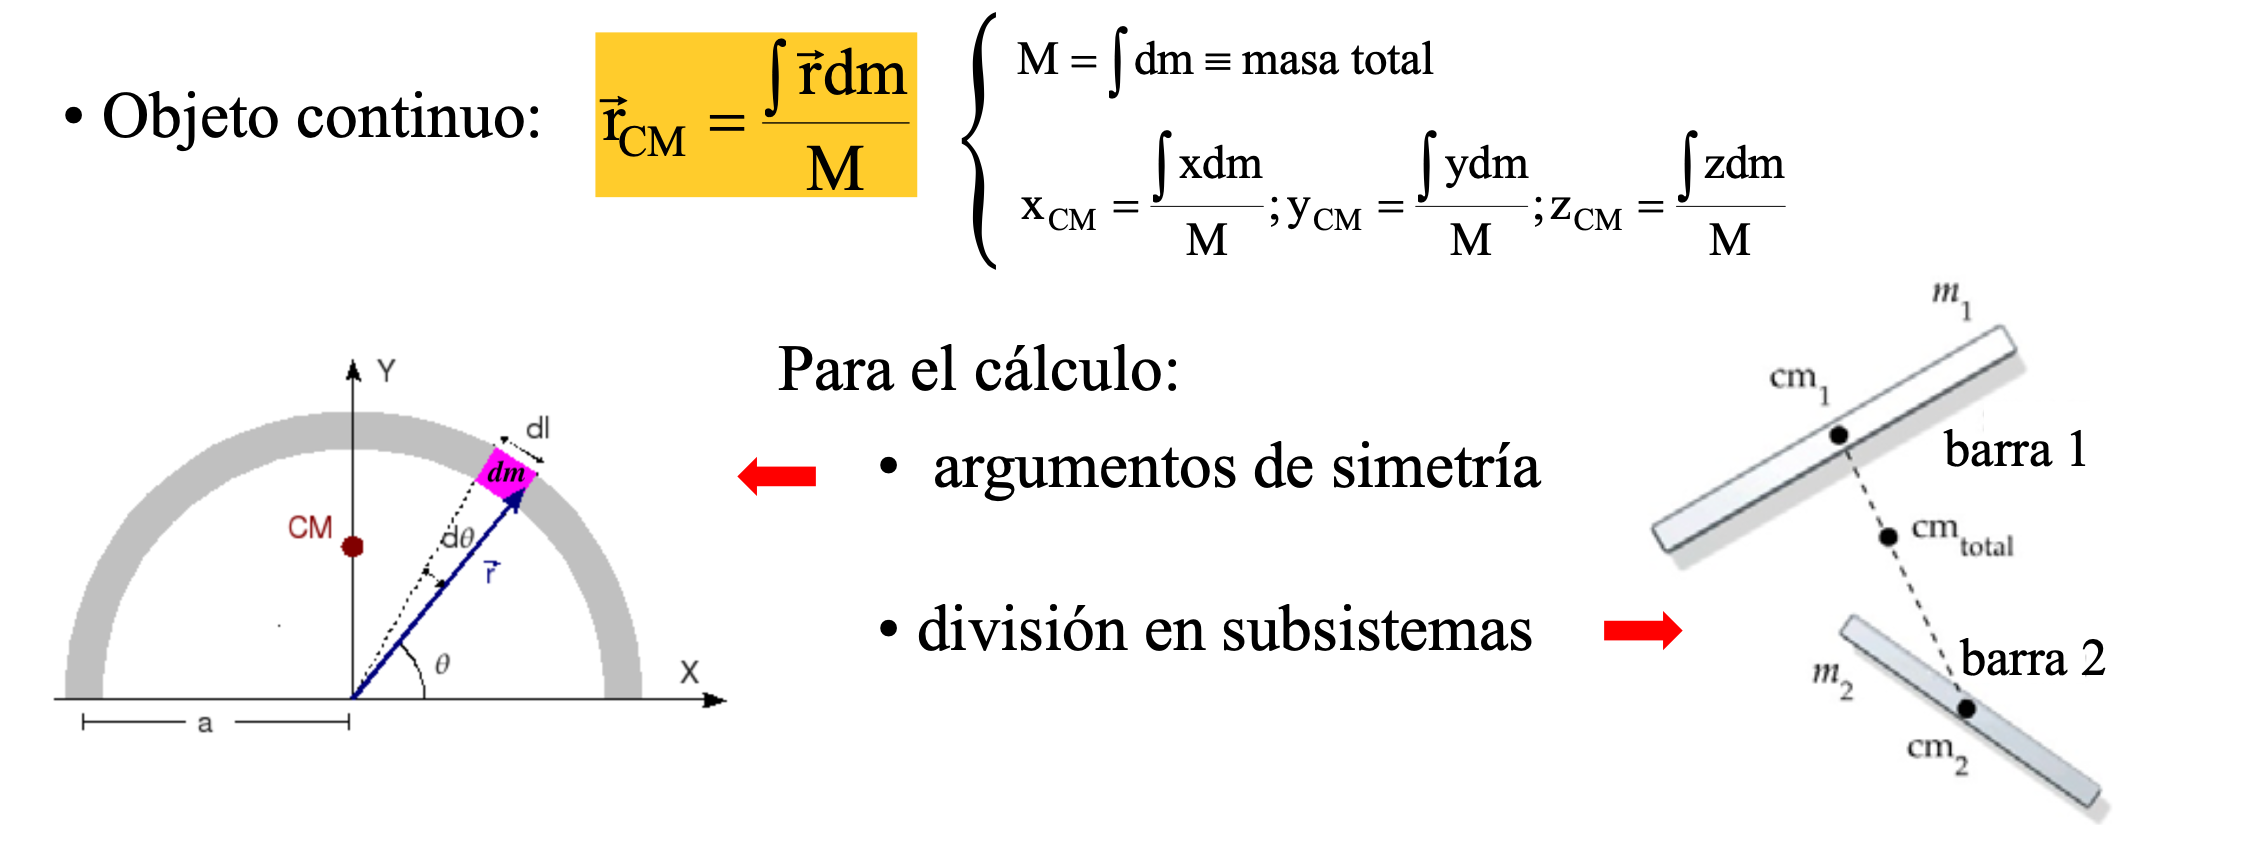
\includegraphics[width=1\textwidth]{imagenes/imagenes12/T12IM02.png}
\end{figure}

\begin{figure}[H]
	\centering
	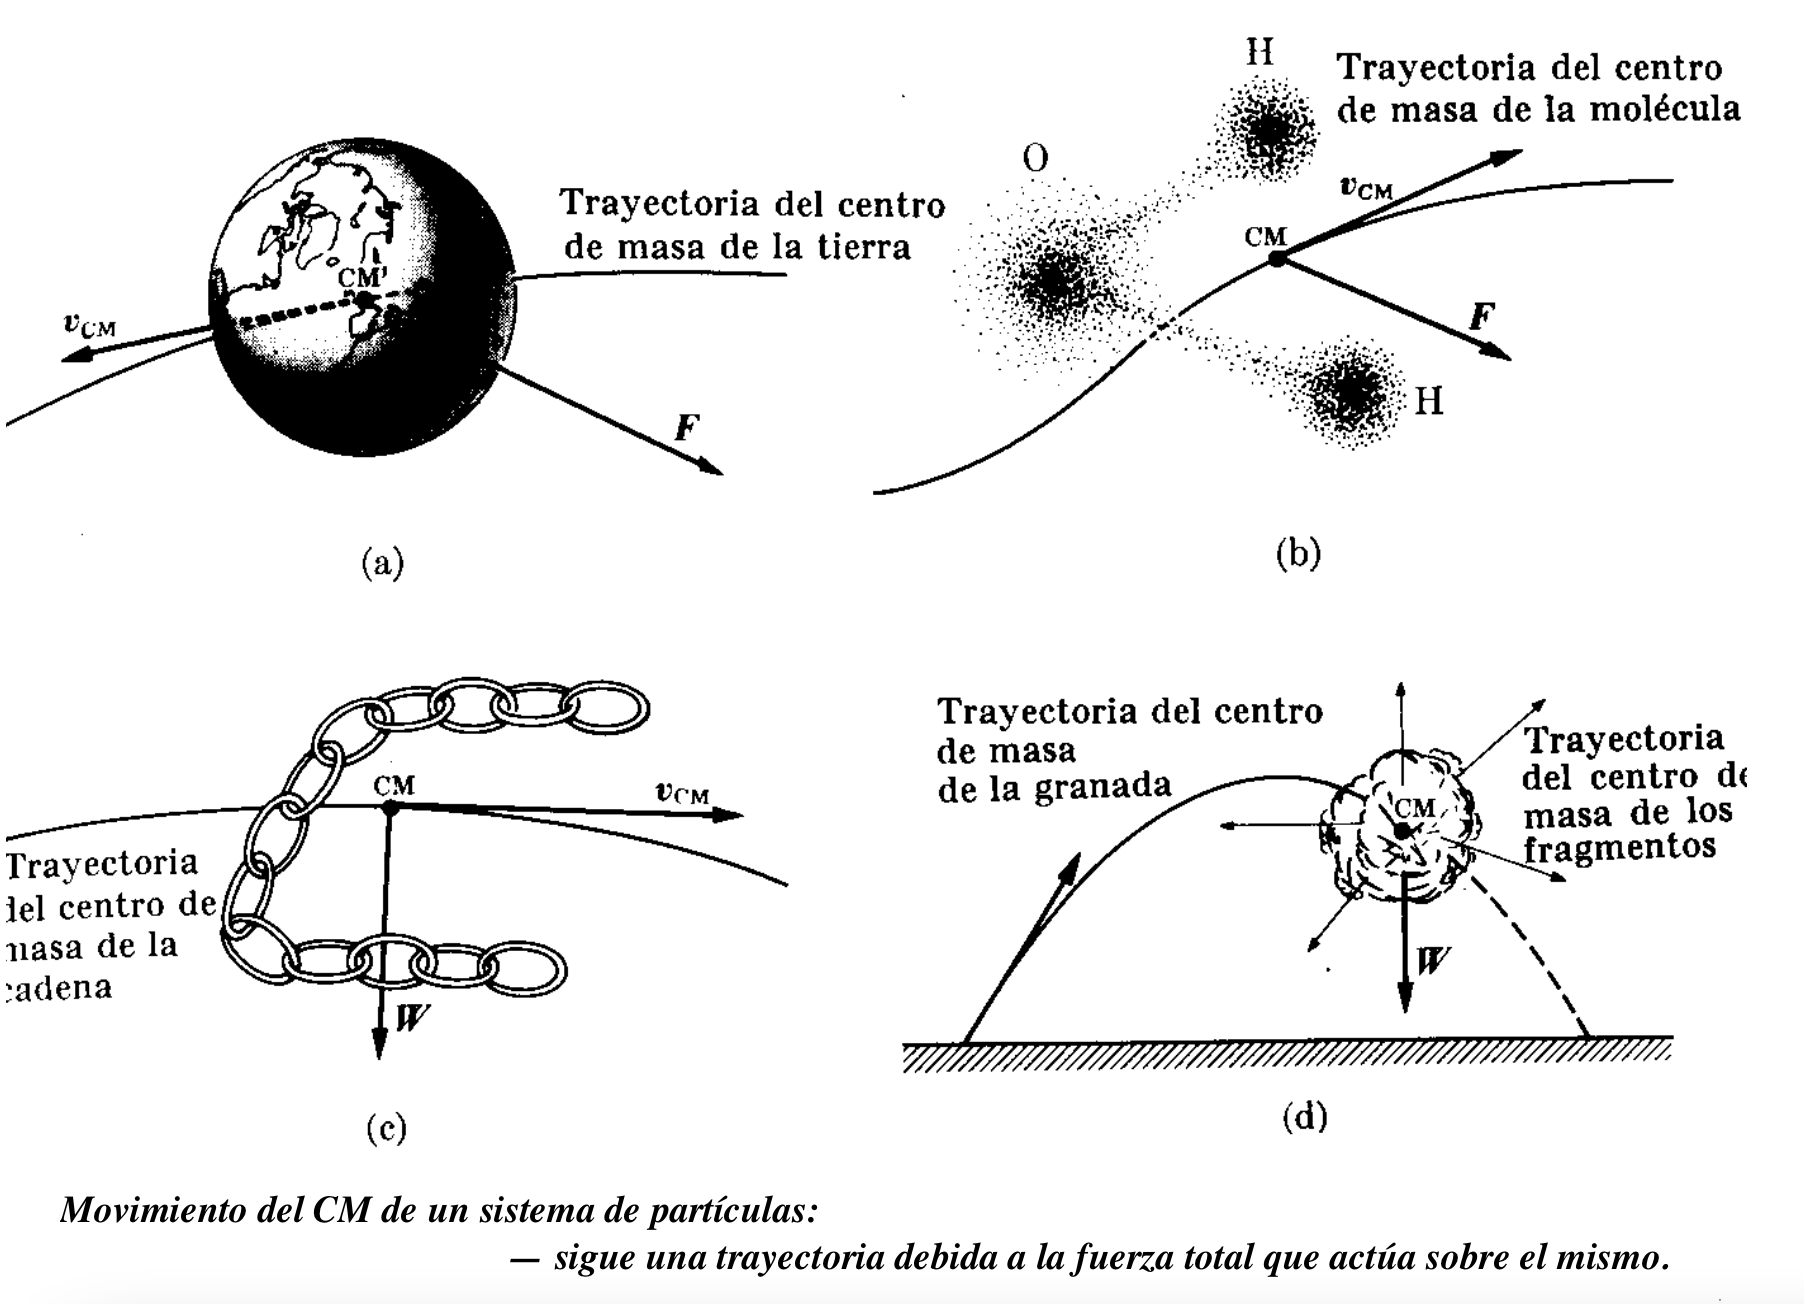
\includegraphics[width=1\textwidth]{imagenes/imagenes12/T12IM05.png}
\end{figure}



\section[Momento Cinético. Teorema de König. Teorema del momento angular]{Momento Cinético. Teorema de König. Teorema del momento angular\sectionmark{Teorema del momento angular}}
\sectionmark{Teorema del momento angular}

\textcolor{gris}{ \textsf{ \small{Momento cinético = momento angular}\normalsize{.} } }

\begin{multicols}{2}
$\vec L_i=\vec r_i \times m\vec v_i$

$\vec L =\displaystyle \sum_{i_1}^N \vec L_i  = \sum_{i=1}^N\vec r_i \times m\vec v_i$

$\boldsymbol{\vec r_i=\overrightarrow R + \vec r_{i,CM}}$

Derivando respecto al tiempo:

$\vec v_i=\vec v_{CM}+\vec v_{i,CM}$
\begin{figure}[H]
	\centering
	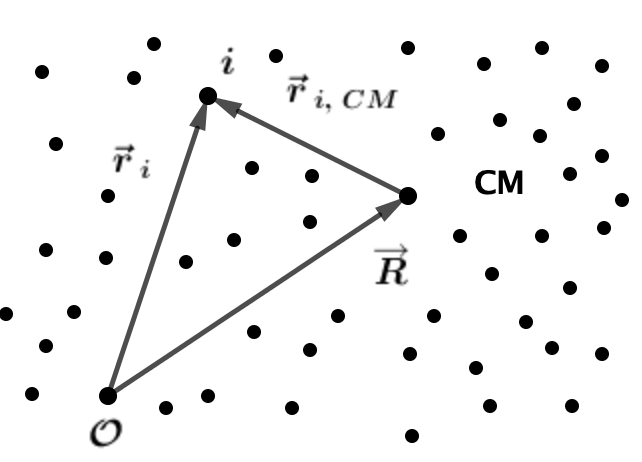
\includegraphics[width=.4\textwidth]{imagenes/imagenes12/T12IM03.png}
\end{figure}
\end{multicols}

Sustituyendo en la expresión de $\vec L$:

$\vec L =\displaystyle \sum_{i=1}^N\vec r_i \times m \ \vec v_i =
\sum_{i=1}^N \  m_i\ \left[ \ ( \ \vec R +\vec r_{i,CM} \ ) \ \times \ ( \ \vec v_{CM}+\vec v_{i,CM} \ ) \ \right]$

$\vec L = \displaystyle \sum_{i=1}^N \left( 
m_i \vec R \times \vec v_{CM}+m_i \vec R \times \vec v_{i,CM}+m_i \vec r_{i,CM} \times \vec v_{CM}  +m_i \vec r_{i,CM} \times  \vec v_{i,CM}
\right)=$

\small{$\displaystyle =
\vec R \times M\  \vec v_{CM}+\vec R \times \sum_{i=1}^N m_i \vec v_{i,CM}+   \left( \sum_{i=1}^N  m_i \vec r_{i,CM} \right) \times \vec v_{CM}  +  \sum_{i=1}^N   \vec r_{i,CM} \times m_i \vec v_{i,CM}
$}\normalsize{$=$}

Como, 

\hspace{7mm} $\  \ \displaystyle \vec R \times \sum_{i=1}^N m_i \vec v_{i,CM}=\vec R \times \cancelto{0}{\vec P_{CM}}=0 \ $ (cantidad de movimiento del CM respecto al CM) y
  
\hspace{7mm} $\displaystyle  \left( \sum_{i=1}^N  m_i \vec r_{i,CM} \right) \times \vec v_{CM} =0\ $ (posición del CM respecto al CM), 

finalmente:

\begin{equation}
\subrayado{\ \boxed{\  \boldsymbol{ \vec L \ =\ \vec R \times M \ \vec v_{CM}\ + \ \sum_{i=1}^N \ \vec r_{i,CM} \times m_i \ \vec v_{i,CM} }\ }\ }
\end{equation}

\begin{miparrafodestacado}
El \textbf{teorema de König} dice que el momento angular de un sistema de $N$ partículas es la suma de dos térmicos o contribuciones:
\begin{itemize}
\item primer término: momento angular de una sola partícula de masa $M$, la masa total del sistema, desplazándose a la velocidad del centro de masas, $\vec v_{CM}$
\item  Momento angular relativo de las N partículas respecto el $CM$.
\end{itemize}
\end{miparrafodestacado}

$$\subrayado{\ \boxed{\ \boldsymbol{\overrightarrow{L}=\overrightarrow{L}_{CM}+\overrightarrow{L}_{Rel}}\ }\ }$$
\vspace{-8mm} %***************************************
\begin{figure}[H]
	\centering
	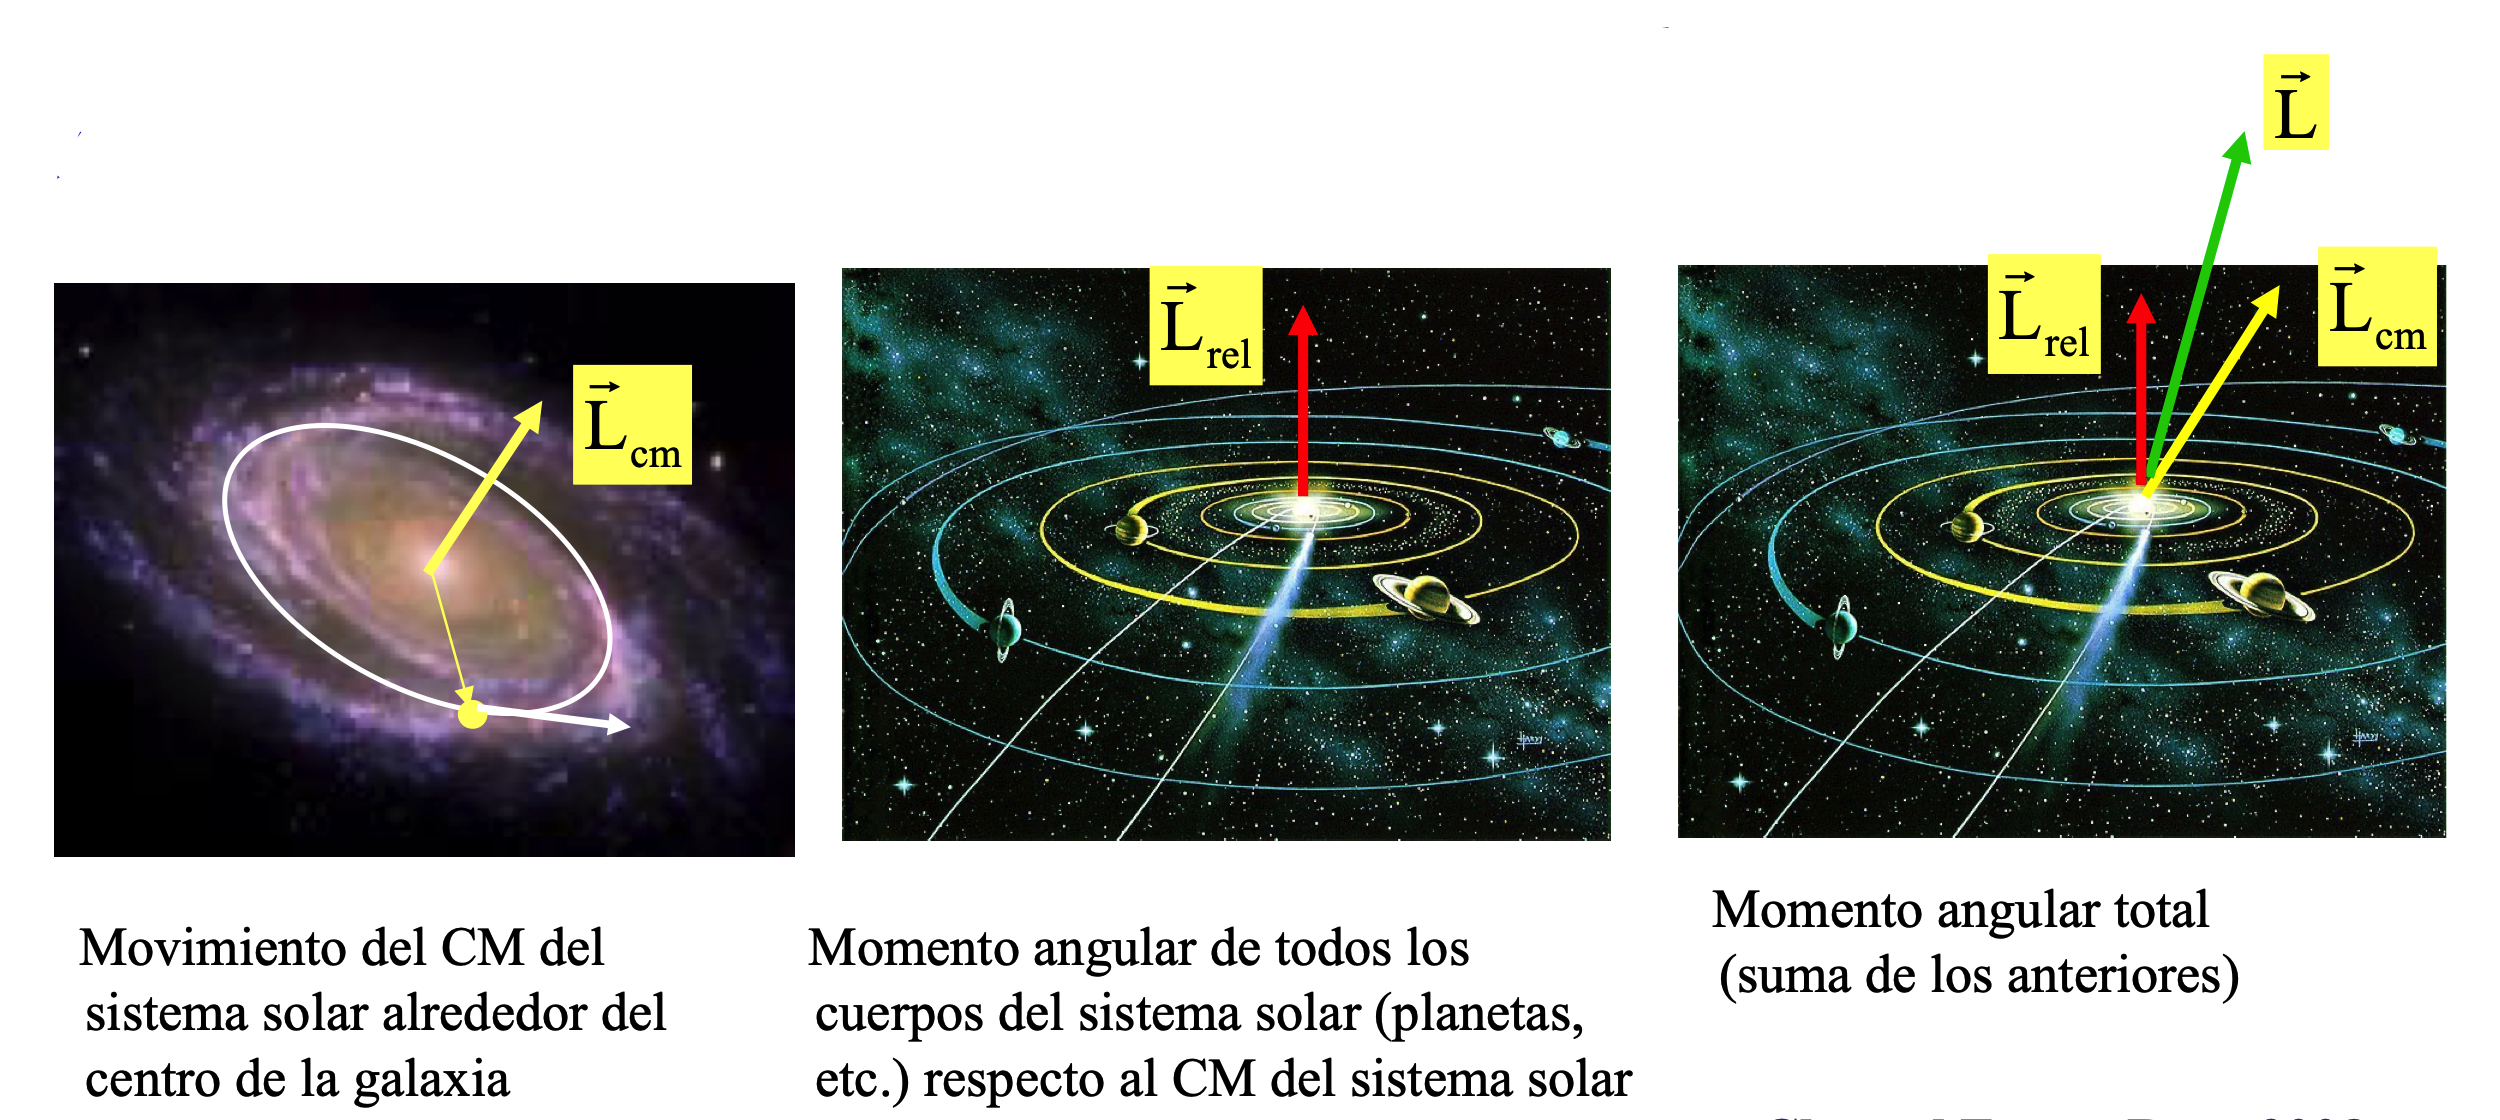
\includegraphics[width=1\textwidth]{imagenes/imagenes12/T12IM04.png}
\end{figure}


\textbf{Teorema del momento angular}, veamos como varía el momento angular con el tiempo:

$ \displaystyle  \dv{\vec L}{t} =\dv{t} \sum_{i=1}^N m_i \vec r_i \times \vec v_i= \cancelto{0,\text{ \tiny{paralelos}}}{\sum_i \vec v_i \times m_i \vec v_i} + \sum_i{ \vec r_i \times m_i \dv{\vec v_i}{t} } $

Teniendo en cuenta la segunda ley de Newton,

$ \displaystyle  \dv{\vec L}{t}=\sum_i \vec r_i \times \left[ 
\sum_j \vec F_{ji} \ + \ \vec F_i^{(e)}
\right]$

Luego:

$ \displaystyle  \dv{\vec L}{t}=\sum_i \sum_j \vec r_i \times \vec F_{ji}\ + \ \sum_i \vec r_i \times \vec F_i^{(e)}$

Por la tercera de Newton (acción y reacción) $\vec F_{ji}=-\vec F_{ij}$, aparecen $N$ parejas del tipo: $\vec r_i\times \vec F_{ji}+ \vec r_j \times \vec F_{ij}=(\vec r_i - \vec r_i)\times \vec F_{ji}=\vec r_{ji}\times \vec F_{ji}=0$, al ser vectores paralelos. Con ello:
\vspace{-3mm} %**********************************************
\begin{equation}
	\subrayado{\ 
	\boxed{\ \boldsymbol{
	\dv{\overrightarrow L}{t}\ =\ \overrightarrow{M}^{(e)}
	}
	\ }
	\ }
	\ ; \qquad
	\text{ siendo } \ \overrightarrow{M}^{(e)}=\sum_i \vec r_i \times \vec F_i^{(e)}
\end{equation}
\vspace{-7mm}  %**********************************************
\begin{miparrafodestacado}
En el caso particular de que $\overrightarrow{M}^{(e)}=0 \ \to \ \overrightarrow{L}=\overrightarrow{cte}$, el momento angular total del sistema será un vector constante.
\end{miparrafodestacado}

\section{Teorema de la energia}


Supongamos que tenemos una particula que cambia de una configuración $1$ a una configuración $2$; entonces, el trabajo efectuado será:
$ \int_1^2 \vec F_i \cdot \dd \vec r_i$, para el sistema de $N$ partículas:

$ \displaystyle W_{12}= \sum_{i=1}^N \int_1^2 \vec F_i \cdot \dd \vec r_i= \sum_{i=1}^N \int_1^2 m_i \ \dv{\vec v_i}{t} \cdot \vec v_i \ \dd t = \sum_{i=1}^N \int_1^2 m_i \ \vec v_i \cdot \dd \vec v_i = $

Como $\vec v \cdot  \dd \vec v= v \dd v$, tendremos que 

$\boldsymbol{ W_{12} }=\displaystyle \sum_{i=1}^N \int_1^2 m_i \  v_i \ \dd  v_i = \sum_{i=1}^N \int_1^2 \dd \left( \dfrac 1 2 m_i v_i^2 \right)= \sum_{i=1}^N \left[ \ \mathcal E_{c_i}(2)-\mathcal E_{c_i}(1) \ \right] = \boldsymbol{ \mathcal E_c(2)-\mathcal E_c(1) }, \ $ 

donde $\mathcal E_c(c)=\displaystyle \sum_{i=1}^N \dfrac 1 2 m_i v_i^2 \ $ es la energía cinética del sistema en una configuración dada $c$.

$\vec r_i=\vec R + \vec r_{i,CM}  \to  \vec v_i=\vec v_{CM}+\vec v_{i,CM}  \to  v_i^2=v_{CM}^2 +v_{i,CM}^2 +2v_{CM}v_{i,CM}$

$\mathcal E_c(c)=\displaystyle \sum_{i=1}^N \dfrac 1 2 m_i v_i^2 = \sum_{i=1}^N \dfrac 1 2 m_i \left( v_{CM}^2 +v_{i,CM}^2 +2v_{CM}v_{i,CM} \right)$

$\mathcal E_c(c)=\displaystyle \dfrac 1 2 M  v_{CM}^2 + \sum_{i=1}^N \dfrac 1 2 m_i v_{i,CM}^2 + 2 \frac 1 2 \ v_{CM}\ \cancelto{0, {\text{\tiny{P respecto CM}}}}{\sum_{i}m_i v_{i,CM}}=0$

\begin{equation}
\subrayado{\ 
	\boxed{\ \boldsymbol{
\mathcal E_c(c)=\displaystyle \dfrac 1 2 M  \ v_{CM}^2 \ + \ \sum_{i=1}^N \dfrac 1 2 \ m_i \ v_{i,CM}^2
	}
	\ }
	\ }
\end{equation}

\textbf{Teorema de König de la energía para un sistema de $N$ partículas.}

\begin{miparrafodestacado}
La energía cinética total del sistema de partículas es igual a la energía cinética de una partícula de masa la total del sistema, $M$, que se desplaza a la velocidad del centro de masas, $v_{CM}$ más las energías cinéticas de todas las partículas medidas respecto del centro de masas.
\end{miparrafodestacado}

Por otra parte, como

$W_{12}=\displaystyle \sum_{i=1}^N \vec F_i \cdot \dd \vec r_i= 
\sum_{i=1}^N \int_1^2 \left[ \vec F_i^{(e)}+\sum_j \vec F_{ji} \right] \cdot \dd \vec r_i=$

$= \displaystyle \sum_{i_i}^N \int_1^2 \vec F_i^{(e)} \dd \vec r_i + \sum_i \sum_j \int_1^2 \vec F_{ji} \dd \vec r_i =
W_{ext}+ W_{int} \quad \to $



$$\subrayado{\ \boldsymbol{ \mathcal E_c(2)\ -\ \mathcal E_c(1)=W_{ext}\ +\ W_{int} } \ }$$

Que es el \textbf{teorema más general de la energía}.

Vamos a imponer unas restricciones al sistema. Los resultados que obtengamos serán aplicables solo a sistemas que cumplas esas restricciones.

------ Desarrollemos primero el trabajo realizado por las fuerzas interiores:


$\displaystyle W_{int}=\sum_i \sum_j \int_1^2 \vec F_{ji} \cdot \dd \vec r_i =\sum_i { \int_1^2 \left( \vec F_{1i} \cdot \dd \vec r_i +  \vec F_{2i} \cdot \dd \vec r_i + \cdots + \vec F_{Ni} \cdot \dd \vec r_i   \right)  }$

donde aparecen $N$ parejas del tipo $\vec F_{ij} \cdot \dd \vec r_i + \vec F_{ji} \cdot \dd \vec r_j  $

\textbf{Primera hipótesis:} \emph{Las fuerzas interiores que intervienen cumplen la tercera ley de la dinámica}, ley de acción y reacción: $\vec F_{ij}=-\vec F_{ji}$.

$\vec F_{ij} \cdot \dd \vec r_i + \vec F_{ji} \cdot \dd \vec r_j= \vec F_{ij}\cdot (\dd \vec r_i - \dd \vec r_j)=\vec F_{ij}\cdot \dd \vec r_{ij}  $

\textbf{Segunda hipótesis:} \emph{Admitimos que las fuerzas interiores son conservativas.}

$\vec F_{ij}=-\overrightarrow{\grad}\mathcal E_{p_{ij}} \to \vec F_{ij}\cdot \dd \vec r_{ij}=-\overrightarrow{\grad}\mathcal E_{p_{ij}}\cdot \dd \vec r_{ij}$

\small{ $\dd \vec r_{ij} \cdot \overrightarrow{\grad}\mathcal E_{p_{ij}}= \displaystyle
 \left( \vec i \ \pdv{\mathcal E_{p_{ij}}}{x_{ij}} + 
        \vec j \ \pdv{\mathcal E_{p_{ij}}}{y_{ij}}
        \vec k \ \pdv{\mathcal E_{p_{ij}}}{z_{ij}}   \right) \cdot  
 \left( \vec i \dd x_{ij} + \vec j \dd y_{ij} + \vec k \dd z_{ij} \right) =\dd \mathcal E_{p{ij}}$}
 
 \normalsize{$\vec F_{ij}\cdot \dd \vec r_{ij}=-\overrightarrow{\grad}\mathcal E_{p_{ij}}\cdot \dd \vec r_{ij}=-\dd \mathcal E_{p_{ij}}$}


\textcolor{gris}{Hemos usado que: $\ f(x,y,z)\to \ \displaystyle \pdv{f}{x}\dd x+ \pdv{f}{y} \dd y + \pdv{f}{z} \dd z \ = \ \dd f$}

$W_{int}=\displaystyle -\sum_i \sum_j \int_1^2 \vec F_{ij} \cdot \vec \dd r_{ij}=-\sum_i \sum_{j>i} \int_1^2 \dd \mathcal E _{p_{ij}}$

\textcolor{gris}{Hemos usado $j>i$ para asegurar $j\neq i$}

Luego, para fuerzas interiores conservativas que cumplan la tercera ley de la mecánica (acción y reacción):

$\displaystyle \boldsymbol{ W_{int}=} -\eval{\sum_i \sum_{j>i} \ \mathcal E_{p_{ij}}}_1^2= -\left( \mathcal E_{p,int}(2)-\mathcal E_{p,int}(1) \right) \boldsymbol{ =\mathcal E_{p,int}(1)-\mathcal E_{p,int}(2) }$

Sustituyendo en el teorema general de la energía,

$\displaystyle 
\left[ \  \mathcal E_c(2) + \mathcal E_{p,int}(2) \  \right  ]-
\left[ \  \mathcal E_c(1) + \mathcal E_{p,int}(1) \  \right  ] \ = \
W_{ext}$


Llamando $\subrayado{ \ \boldsymbol{\mathcal U(c)=\mathcal E_c(c) + \mathcal E_{p,int}(c)} \ }$, \colorbox{LightYellow}{\textbf{\emph{energía propia}}} de la configuración c, podemos escribir:

$$\boldsymbol{\mathcal U(2)-\mathcal U(1)=W_{ext}}$$

------ Vamos, ahora, a por el trabajo de las fuerzas externas.

\textbf{Tercera hipótesis:} \emph{Supongamos que también las fuerzas exteriores son conservativas}

\textcolor{gris}{Cada vez que añadimos hipótesis restringimos más el problema.}

$\boldsymbol{\vec F_i^{e}=-\overrightarrow{\grad}\mathcal E_{p_{i,ext}}}$

$\displaystyle W_{ext}=\sum_i \int_1^2 \vec F_i^{e} \cdot \dd \vec r_i=-\sum_i \int_1^2 \overrightarrow{\grad} \mathcal E_{p_{i,ext}} \cdot \dd \vec r_i=-\sum_i \int_1^2 \dd \mathcal E_{p_{i,ext}}=\mathcal E_{p, ext}(1)-\mathcal E_{p,ext}(2)$ 

Substituyendo, también, en la ecuación del teorema general de la energía, obtenemos que en el caso de que las fueras externas cumplan la tercera ley de Newton (acción-reacción) y que las fuerzas internas y externas sean conservativas:

\begin{equation}
\subrayado{
\boldsymbol{ 
	\left[ \mathcal E_c(2) + \mathcal E_{p,int}(2)+ \mathcal E_{p,ext}(2)  \right]    -  \left[ \mathcal E_c(1) + \mathcal E_{p,int}(1)+ \mathcal E_{p,ext}(1) \right]   =  0
	}
	}
\end{equation}

Si llamamos $ \mathcal E_c(c) + \mathcal E_{p,int}(c)+ \mathcal E_{p,ext}(c) = E(c)$, energía total del sistema en el estado $c$, 


\begin{equation}
\subrayado{\boldsymbol{ \ E \ = \ cte\ }}	
\end{equation}

Muchos autores llaman a este resultado \emph{principio de conservación de la energía}, pero no se trata de un principio sino de un teorema basado en las tres leyes de Newton de la mecánica. Es un caso particular (\footnotesize{en que las fueras externas cumplen la tercera ley de Newton (acción-reacción) y que las fuerzas internas y externas son conservativas}) \normalsize{que} se suele presentar en casos macroscópicos.


\section{Problemas}

\begin{prob}
Una granada que cae verticalmente explota en dos fragmentos de igual masa cuando se encuentra a una altura de $2000 \ \mathrm{m}$ y tiene una velocidad hacia abajo de $$60\ \mathrm{m \ s}^{-1}$$. Inmediatamente después de la explosión, uno de los fragmentos se mueve hacia abajo con velocidad $80\ \mathrm{m \ s}^{-1}$	. Encontrar la posición del centro de masas pasados $10\ \mathrm{s}$ de la explosión.
\end{prob}

--- Primer método:

Como resultado de la explosión, las fuerzas exteriores no cambian. El $CM$ continuará moviéndose en línea recta como si no hubiese ocurrido la explosión. Por ello, estará a una distancia $y=y_0+v_0t+\frac 1 2 g t^2$, con $y_0=200\mathrm{m}$, $v_0=-60\ \mathrm{m \ s}^{-1}$, $g=-9.8  \mathrm{m \ s}^{-2}$, con lo que para $t=10\ \text{s}$ se obtiene $\boldsymbol{y_{CM}=910\ \text{m}}$.

--- Segundo método:

Podemos encontrar la posición del centro de masa a partir de las posiciones de los dos fragmentos iguales en que se divide la granada al explotar. Como $\vec F^{(e)}=\vec 0 \ \to \ \displaystyle \sum_i \vec p_i=\overrightarrow{cte}$ y la cantidad de movimiento se conserva.

En el momento de la explosión, $mv_0=m_1v_1+m_2v_2$, 

como $m_1=m_2=\frac 1 2 m$, luego $2v_0=v_1+v_2$, resulta que

$v_0=-60\ \mathrm{m \ s}^{-1};\ v_1=-80\ \mathrm{m \ s}^{-1} \to \ v_2=-40\ \mathrm{m \ s}^{-1}$

Después de $10 \ \text{s}$ de la explosión, cada fragmento se encuentra en la posición $y_i=y_{0i}+v_it+\frac 1 2 g t^2$, con $y_{01}=y_{02}=2000\ \text{m}$, $v_1=-80\ \mathrm{m \ s}^{-1}$, $v_2=-40\ \mathrm{m \ s}^{-1}$, $g=-9.8  \mathrm{m \ s}^{-2}$, $t=10\ \text{s}$, sustituyendo: $y_1=710\ \text{m}$ e $y_2=110\ \text{m}$

El $CM$ estará en: $\boldsymbol{y_{CM}}=\dfrac{\frac 1 2 m \ y_1 + \frac 1 2 m \ y_2}{m}= \dfrac 1 2 (y_1+y_2)=\boldsymbol{910\ \text{m}}$


\begin{prob}.
	\begin{figure}[H]
	\centering
	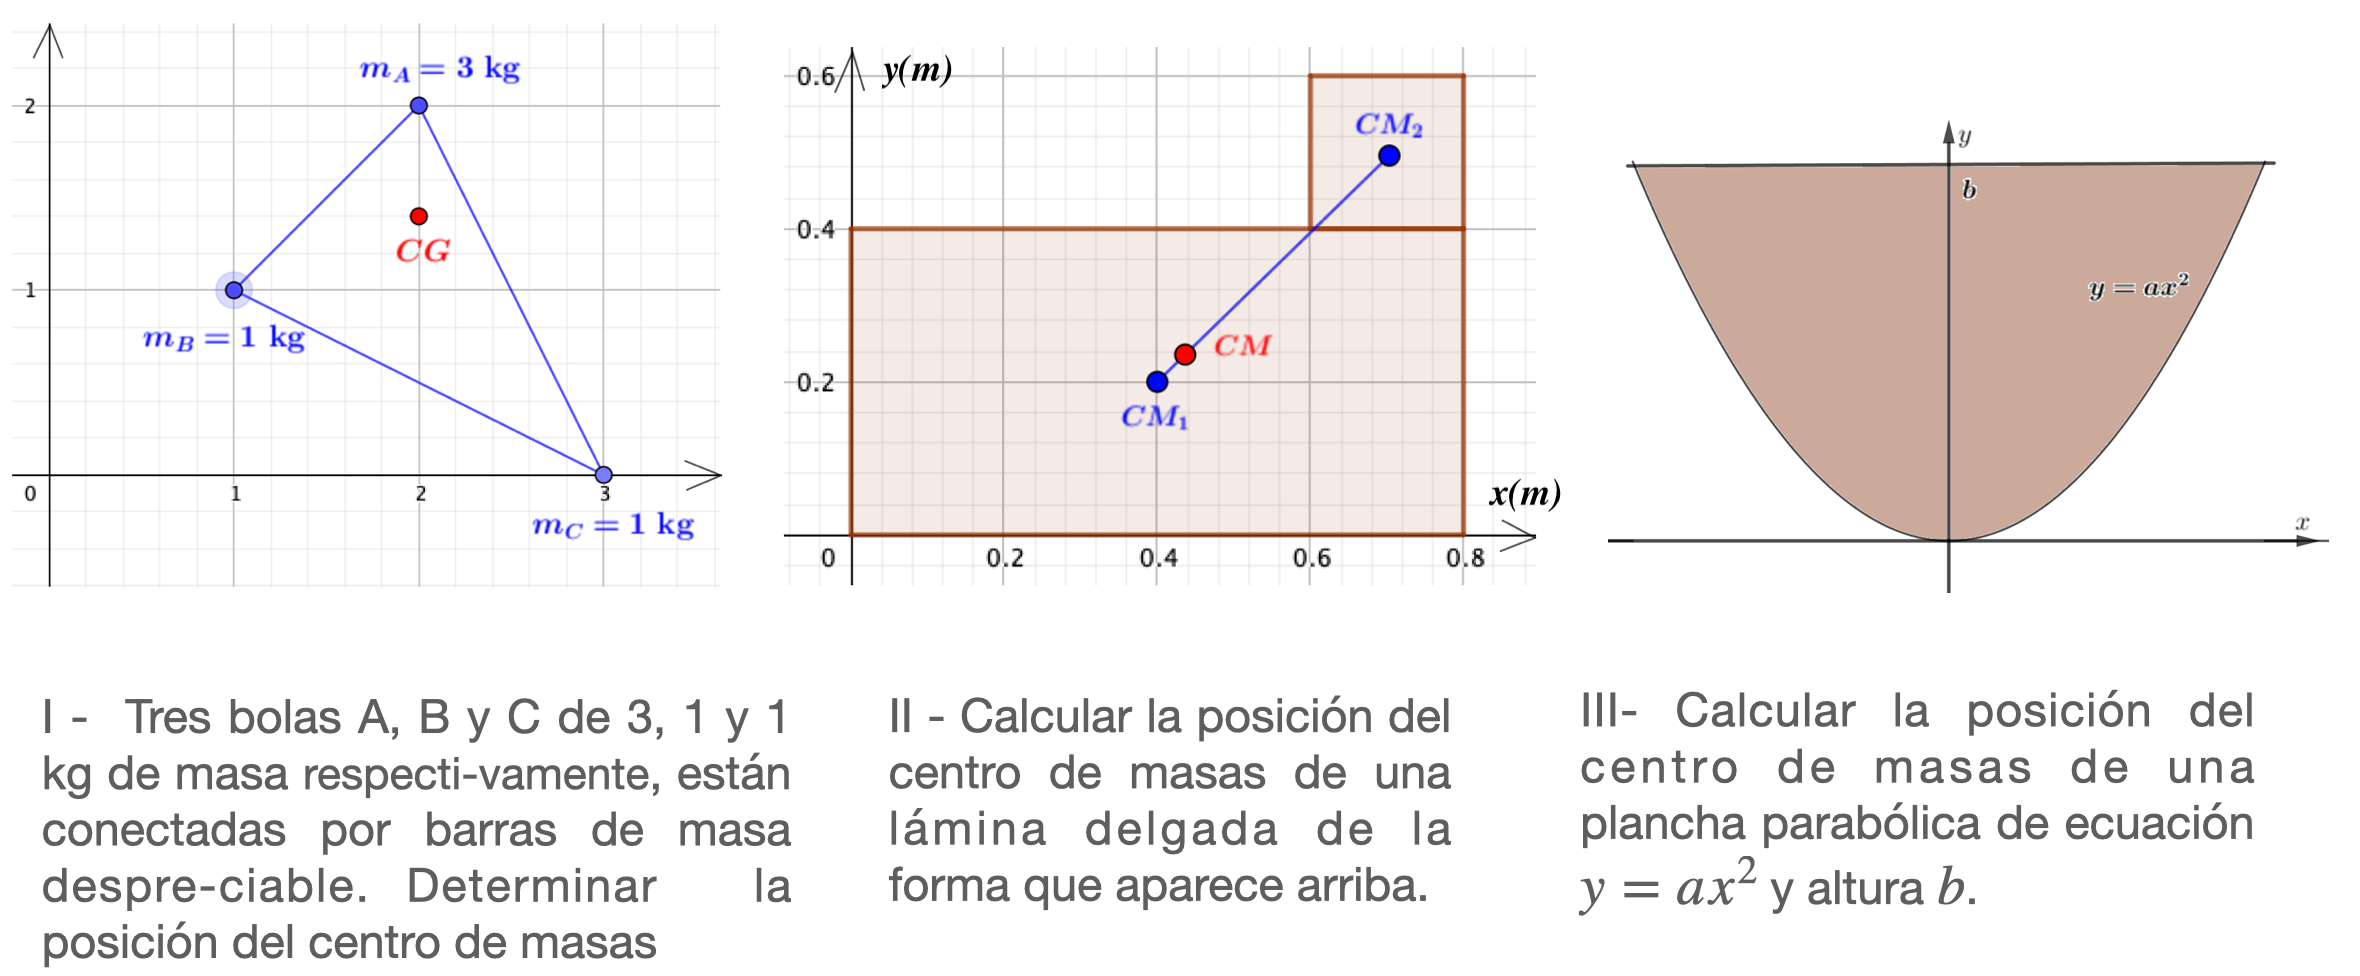
\includegraphics[width=1\textwidth]{imagenes/imagenes12/T12IM06.png}
\end{figure}
\end{prob}

------ Figura I:

$\vec R_{CM}=(x_{CM},y_{CM})=\dfrac {3((2,2)+1(1,1)+1(3,0)}{3+1+1}=\left( 2, \dfrac 7 5 \right)$

------ Figura II:

Para cuerpos planos  con la masa $M$ uniformemente distribuida en un área $A$, se define la densidad superficial uniforme de carga como $\sigma =\frac M A$. 

Así, podemos considerar nuestro cuerpo como formado por dos: el primero, rectángulo grande, de masa  $m_1= \sigma A_1=\sigma  \ 0.4 \times 0.8=0.32 \ \sigma\  \text{kg}$ situado en su centro de gravedad , que por simetría, $CM_{1}=(0.4,0.2)\ \text{m}$. Con un razonamiento análogo: $m_2=\sigma \ 0.2 \times 0.2=0.04 \ \sigma \ \text{kg}$ situado en $CM_2=(0.6+0.1, 0.4+0.1)=(0.7,0,5)\ \text{m}$

Usando la misma fórmula anterior: $(x_{CM},y_{CM})=(0.43,0.26)\ \text{m}$

--- Figura III

Para superficies continuas con densidad superficial uniforme $\sigma=\frac M A$:

$\displaystyle \vec R_{CM}=(x_{CM},y_{CM})=\dfrac 1 M \int \vec r \ \dd m
= \dfrac 1 {\cancel{\sigma} \ A} \int \vec r \ \cancel{\sigma} \dd A= \dfrac  1 A \int \vec r \ \dd A=
\dfrac 1 A \int (x,y) \ \dd A $

Luego, $\displaystyle \quad x_{CM}=\dfrac 1 M \int x \dd m;\qquad y_{CM}=\dfrac 1 M \int y \dd m$

Calculemos primero el área $A$ de la placa parabólica. 

\begin{multicols}{2}
Por matemáticas, el área bajo una curva es $\int f(x)\dd x$, pero nosotros estamos interesados en el área por encima de la curva. Este área será igual al área del rectángulo menos el área bajo la curva.

$y=ax^2=b \to x=\pm \sqrt{b/a}$
\begin{figure}[H]
	\centering
	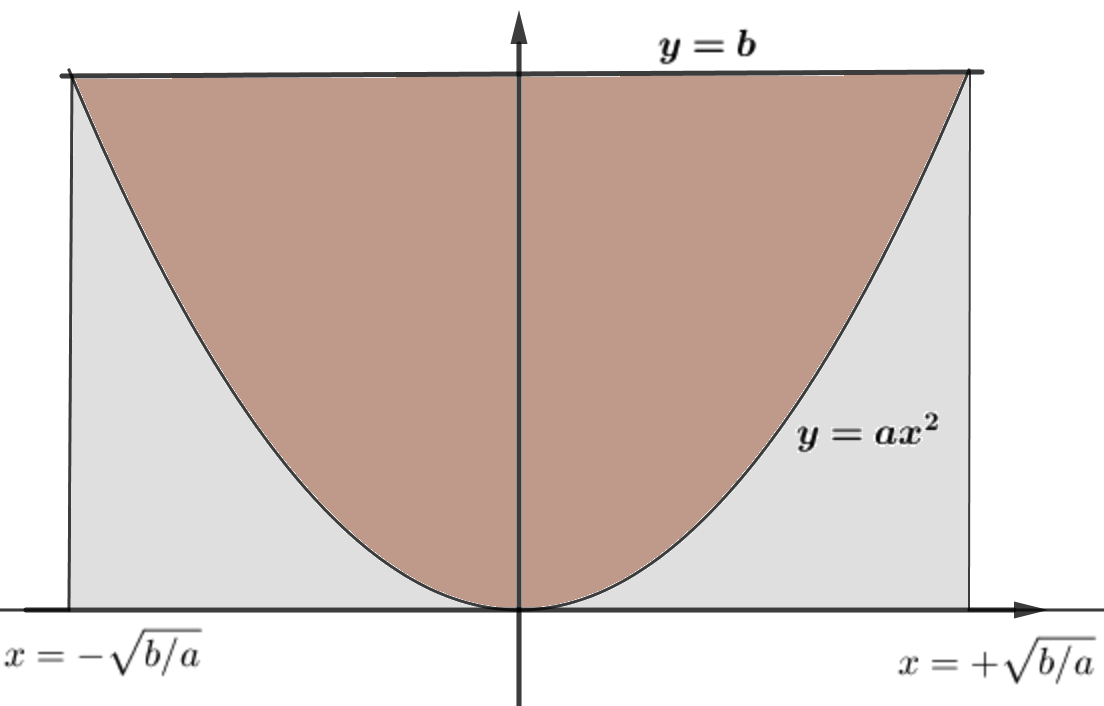
\includegraphics[width=.4\textwidth]{imagenes/imagenes12/T12IM07.png}
\end{figure}
\end{multicols}

Área bajo la curva:
$\displaystyle A=\int_{-\sqrt{b/a}}^{+\sqrt{b/a}} ax^2 dx \eval{a \dfrac {x^3}{3}}_{-\sqrt{b/a}}^{+\sqrt{b/a}}=\dfrac {2b}{3}\sqrt{\dfrac{b}{a}}$

Área del rectángulo: $A_{rectan}=2b\sqrt{\dfrac b a}$

Área de la placa metálica: $\boldsymbol{A}=2b\sqrt{\dfrac b a}- \dfrac{2b}3 \sqrt{\dfrac b a}=\boldsymbol{\dfrac{4b}{3} \sqrt{\dfrac b a}}$

\begin{multicols}{2}
Para calcular la coordenada $x$ del $CM$ será conveniente dividir la placa en diferenciales de área cuyos puntos posean una coordenada $x$ la misma para todos ellos. Vamos por lo tanto a dividir la placa en bandas verticales de espesor $\dd x$. 
\begin{figure}[H]
	\centering
	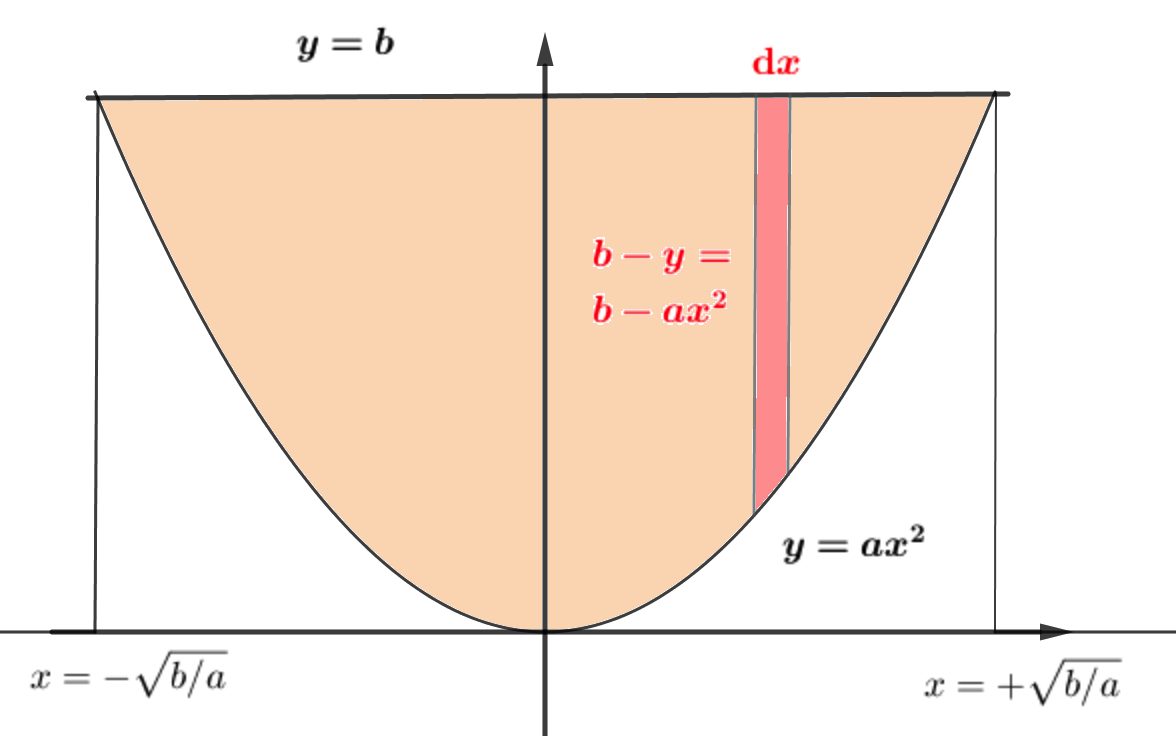
\includegraphics[width=.4\textwidth]{imagenes/imagenes12/T12IM08.png}
\end{figure}
\end{multicols}

$\displaystyle x_{CM}=\dfrac 1 A \int_{-\sqrt{b/a}}^{+\sqrt{b/a}} x \dd A = \dfrac {3}{2b} \sqrt{\dfrac a b} \int_{-\sqrt{b/a}}^{+\sqrt{b/a}} x(b-ax^2) \dd x = $

$=\dfrac {3}{2b} \sqrt{\dfrac a b}\eval{\left( \dfrac {bx^2}{2} - \dfrac  {ax^4}{4} \right) }_{-\sqrt{b/a}}^{+\sqrt{b/a}} = 0$, como era de esperar por la simetría del sistema \textcolor{gris}{Nos hubiésemos podido evitar este cálculo.}

\begin{multicols}{2}
Para calcular la coordenada $y$ del $CM$ sería conveniente dividir la placa en diferenciales de área cuyos puntos poseyeran una coordenada $y$ la misma para todos ellos, es decir en bandas horizontales de espesor $\dd y$. 
\begin{figure}[H]
	\centering
	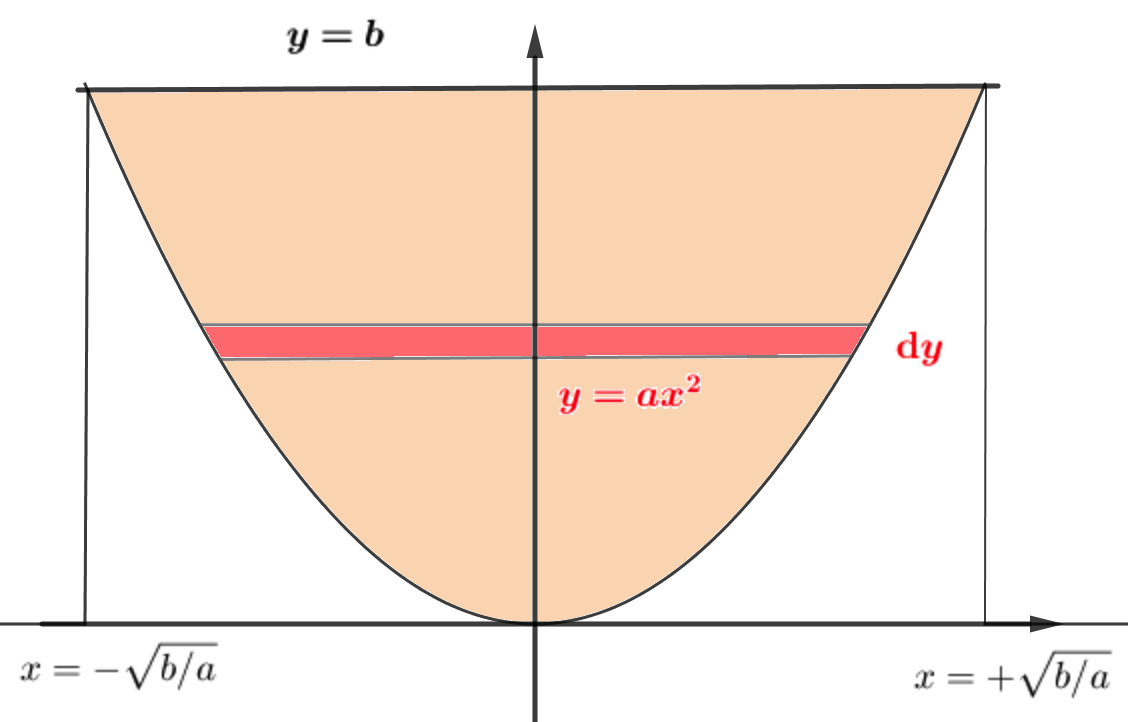
\includegraphics[width=.4\textwidth]{imagenes/imagenes12/T12IM09.png}
\end{figure}
\end{multicols}

$\displaystyle y_{CM}=\dfrac 1 A \int_0^b  y \dd A = \dfrac 1 A\int_0^b y\ 2 \sqrt{\dfrac y a} \dd y = \dfrac {3}{2b} \sqrt{\dfrac a b} \dfrac {2}{\sqrt{a}} \int_0^b y^{3/2} \dd y = $

$= \displaystyle \dfrac{3}{b\sqrt{b}} \eval{\dfrac { 2y^{5/2} } {5} }_0^b=\dfrac{3b}{5}$

Finalmente, el $CM$ de la placa metálica parabólica está en: $\boldsymbol{ \ \left( 0,\dfrac{3b}{5} \right) }$.




\newpage %*************************************
%\begin{comment}
\begin{myblock}{Centro de masas del sistema Tierra - Luna}
 \begin{small}
Vamos a calcular la posición del centro de masas del sistema Tierra-Luna, situando el origen del sistema de referencia en el centro de la Tierra.
 
\vspace{1mm} Los datos que se necesitan para calcularlo son la distancia entre los centros de la Tierra y la Luna, y las masas de ambos cuerpos: 

\vspace{1mm} $d_{TL}= 384100 \ \mathrm{km}:\  M_T= 5.973\times 10^{24} \  \mathrm{kg};\  M_L= 7.349\times 10^{22}\  \mathrm{kg}$

\vspace{1mm} El vector de posición del centro de masas es: 
$\vec r_{CM}=\dfrac{\sum m_i \vec r_i}{\sum m_i}$

\vspace{1mm}  Podemos particularizar para una dimensión, puesto que los centros de la Tierra y la Luna están sobre una línea y después sustituir los datos de la tabla anterior: $r_{CM}=4668\ \mathrm{Km}$

\begin{multicols}{2}
Como el radio de la Tierra es de $6378\ \mathrm{km}$, el centro de masas del sistema Tierra Luna se encuentra debajo de la superficie de la Tierra, como se muestra en la siguiente figura. 
\begin{figure}[H]
	\centering
	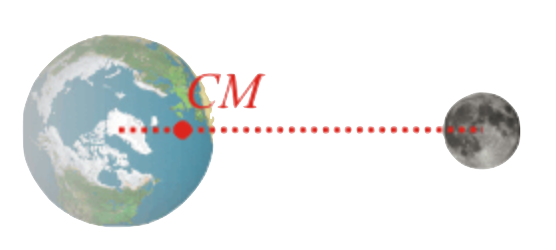
\includegraphics[width=.5\textwidth]{imagenes/imagenes12/T12IM01.png}
\end{figure}

\end{multicols}
Como estamos analizando únicamente el movimiento del sistema Tierra - Luna, podemos considerar que está aislado, por lo que la fuerza gravitatoria que la Tierra ejerce sobre la Luna y su reacción, la fuerza gravitatoria que la Luna ejerce sobre la Tierra, son fuerzas internas y, por tanto, desde el punto de vista de un observador en reposo, el centro de masas del sistema no tiene aceleración (está en reposo). La Luna está orbitando alrededor de la Tierra y, para que el centro de masas del sistema Tierra - Luna permanezca en reposo, el centro de la Tierra ha de estar también en movimiento con respecto a dicho centro de masas. 

\vspace{1mm} Este fenómeno (denominado \emph{wobbling} en inglés) se da entre pares de cuerpos celestes de distinta naturaleza: entre un planeta y su luna (o sus lunas), entre un sol y sus planetas... Dependiendo de las masas de ambos el centro de masas del sistema estará situado entre los dos cuerpos, o bien en el interior de alguno de los dos y, por tanto, el movimiento del sistema de dos cuerpos será diferente en cada caso. El \emph{wobbling} se emplea para detectar planetas que gravitan en torno a estrellas lejanas. 	
\end{small}
\end{myblock}

%\end{comment}










